\documentclass[10pt,aspectratio=169]{beamer}
\usepackage[utf8]{inputenc}
\usepackage[T1]{fontenc}
\usepackage[french]{babel}
\usepackage{amsmath,amssymb,amsfonts,amsthm}
\usepackage{graphicx}
\usepackage{booktabs}
\usepackage{array}
\usepackage{listings}
\usepackage{color}

% Thème Beamer moderne et épuré
\usetheme{Madrid}
\usecolortheme{whale}

% Personnalisation des couleurs pour un rendu premium (Bleu nuit / Ardoise)
\definecolor{brandblue}{RGB}{12, 35, 64}
\definecolor{accentblue}{RGB}{30, 144, 255}
\definecolor{darkslate}{RGB}{47, 79, 79}

\setbeamercolor{palette primary}{bg=brandblue,fg=white}
\setbeamercolor{palette secondary}{bg=accentblue,fg=white}
\setbeamercolor{palette tertiary}{bg=brandblue,fg=white}
\setbeamercolor{titlelike}{parent=palette primary}
\setbeamercolor{structure}{fg=brandblue}
\setbeamercolor{block title}{bg=brandblue,fg=white}
\setbeamercolor{block body}{bg=black!5,fg=black}

\setbeamertemplate{navigation symbols}{} % Supprimer les icônes de navigation de base
\setbeamertemplate{headline}{} % Nettoyer le haut des slides

% Informations sur la présentation
\title[\textbf{Factorisations Incomplètes en Précision Mixte}]{\textbf{Factorisations incomplètes de matrices creuses en précision mixte}}
\subtitle{De l'Analyse Exploratoire à l'Algorithme GEP Mixte}
\author[R. Aouini \& S. Hbabou]{Radouane Aouini \and Sami Hbabou \\ \vspace{0.15cm} \small \textbf{Encadrant :} Théo Mary (LIP6)}
\institute[CCA]{Cryptologie, Calcul haute-performance et Algorithmique (CCA) -- Année Académique 2025-2026}
\date{\today}

\begin{document}

% 1. Slide de Titre
\begin{frame}[plain]
    \titlepage
\end{frame}

% 2. Context & Problématique
\begin{frame}{Introduction \& Problématique}
    \begin{columns}
        \begin{column}{0.55\textwidth}
            \textbf{Le Contexte : Solvers Iteratifs}
            \begin{itemize}
                \item Résolution de $Ax = b$ pour des matrices $A$ très grandes et creuses (milliers à millions de lignes).
                \item Les méthodes de sous-espace de Krylov (ex: \textbf{GMRES}) sont incontournables mais dépendent fortement du conditionnement de $A$.
            \end{itemize}
            \vspace{0.3cm}
            \textbf{Le Préconditionnement ILUT}
            \begin{itemize}
                \item Approximation $A \approx LU = M$.
                \item Le seuil de chute (drop tolerance $\varepsilon$) élimine les éléments mineurs pour limiter le remplissage (\textit{fill-in}).
            \end{itemize}
        \end{column}
        
        \begin{column}{0.45\textwidth}
            \begin{block}{Le goulot d'étranglement Mémoire}
                \begin{itemize}
                    \item $\varepsilon$ strict $\implies$ Forte robustesse / peu d'itérations, mais explosion de la mémoire.
                    \item $\varepsilon$ lâche $\implies$ Faible mémoire, mais convergence lente ou divergence.
                    \item \textbf{Inefficacité du FP64 uniforme} : Stocker tous les éléments proches de zéro en 64 bits est un gaspillage.
                \end{itemize}
            \end{block}
        \end{column}
    \end{columns}
\end{frame}

% 3. L'Approche Proposée : Précision Mixte Adaptative
\begin{frame}{L'Approche Proposée : GEP Mixte}
    \textbf{Objectif :} Compresser drastiquement la taille mémoire du préconditionneur sans dégrader la convergence de GMRES.
    
    \vspace{0.4cm}
    \begin{block}{Le concept GEP Mixte}
        Allouer dynamiquement et à la volée une précision spécifique (parmi 5 niveaux) à chaque élément individuel de la factorisation Incomplète LU en fonction de son impact numérique :
    \end{block}
    
    \vspace{0.2cm}
    \begin{columns}
        \begin{column}{0.2\textwidth}
            \centering
            \textbf{FP16 (Half)} \\ 16-bit \\ $\text{u} \approx 4.8 \times 10^{-4}$
        \end{column}
        \begin{column}{0.2\textwidth}
            \centering
            \textbf{FP24 (Custom)} \\ 24-bit \\ $\text{u} \approx 1.5 \times 10^{-5}$
        \end{column}
        \begin{column}{0.2\textwidth}
            \centering
            \textbf{FP32 (Single)} \\ 32-bit \\ $\text{u} \approx 5.9 \times 10^{-8}$
        \end{column}
        \begin{column}{0.2\textwidth}
            \centering
            \textbf{FP48 (Custom)} \\ 48-bit \\ $\text{u} \approx 1.4 \times 10^{-11}$
        \end{column}
        \begin{column}{0.2\textwidth}
            \centering
            \textbf{FP64 (Double)} \\ 64-bit \\ $\text{u} \approx 1.1 \times 10^{-16}$
        \end{column}
    \end{columns}
\end{frame}

% 4. Fondements Théoriques : Les Erreurs de Dropping
\begin{frame}{Fondements Théoriques : Bornes d'Erreurs de Dropping}
    \begin{block}{Théorème (Local Dropping Bound)}
        Pour tout élément $(i,j)$ supprimé lors de la factorisation ILUT (avec seuil $\varepsilon$), l'erreur locale introduite satisfait :
        $$|E_{ij}| \le \varepsilon \|A_{\cdot,j}\|_2$$
    \end{block}
    
    \vspace{0.2cm}
    \begin{columns}
        \begin{column}{0.5\textwidth}
            \textbf{Démonstration (Esquisse pour $U$ ($i \le j$)) :}
            \begin{itemize}
                \item Soit $v_{ij} = a_{ij} - \sum_{k=1}^{i-1} \hat{l}_{ik}\hat{u}_{kj}$ la valeur calculée avant le drop.
                \item L'algorithme fixe $\hat{u}_{ij} = 0$ ssi $|v_{ij}| \le \varepsilon\|A_{\cdot,j}\|_2$.
                \item L'erreur vaut :
                $$E_{ij} = (\hat{L}\hat{U})_{ij} - a_{ij} = -v_{ij}$$
                \item D'où directement : $|E_{ij}| \le \varepsilon\|A_{\cdot,j}\|_2$.
            \end{itemize}
        \end{column}
        
        \begin{column}{0.5\textwidth}
            \textbf{Implication fondamentale :}
            \begin{itemize}
                \item Puisque l'on accepte déjà une erreur locale de $\varepsilon\|A_{\cdot,j}\|_2$ en supprimant des coefficients, on peut tolérer une erreur d'arrondi de représentation du même ordre sur les coefficients conservés !
                \item \textbf{C'est le budget d'erreur de la colonne $j$}.
            \end{itemize}
        \end{column}
    \end{columns}
\end{frame}

% 5. Phase 1 : Sensibilité au Seuil de Chute (ILUT standard)
\begin{frame}{Phase 1 : Influence du Seuil de Chute sur la Convergence}
    \begin{columns}
        \begin{column}{0.45\textwidth}
            \textbf{Observations sur la matrice \textit{bcsstk08} :}
            \begin{itemize}
                \item Un seuil très lâche ($\varepsilon = 0.2$) nécessite \textbf{53 itérations} GMRES pour converger.
                \item Un seuil très strict ($\varepsilon = 10^{-4}$) converge extrêmement vite en seulement \textbf{10 itérations}.
                \item La baisse du résidu est monotone mais le nombre d'itérations chute drastiquement avec l'augmentation de la qualité du préconditionneur.
            \end{itemize}
        \end{column}
        
        \begin{column}{0.55\textwidth}
            \centering
            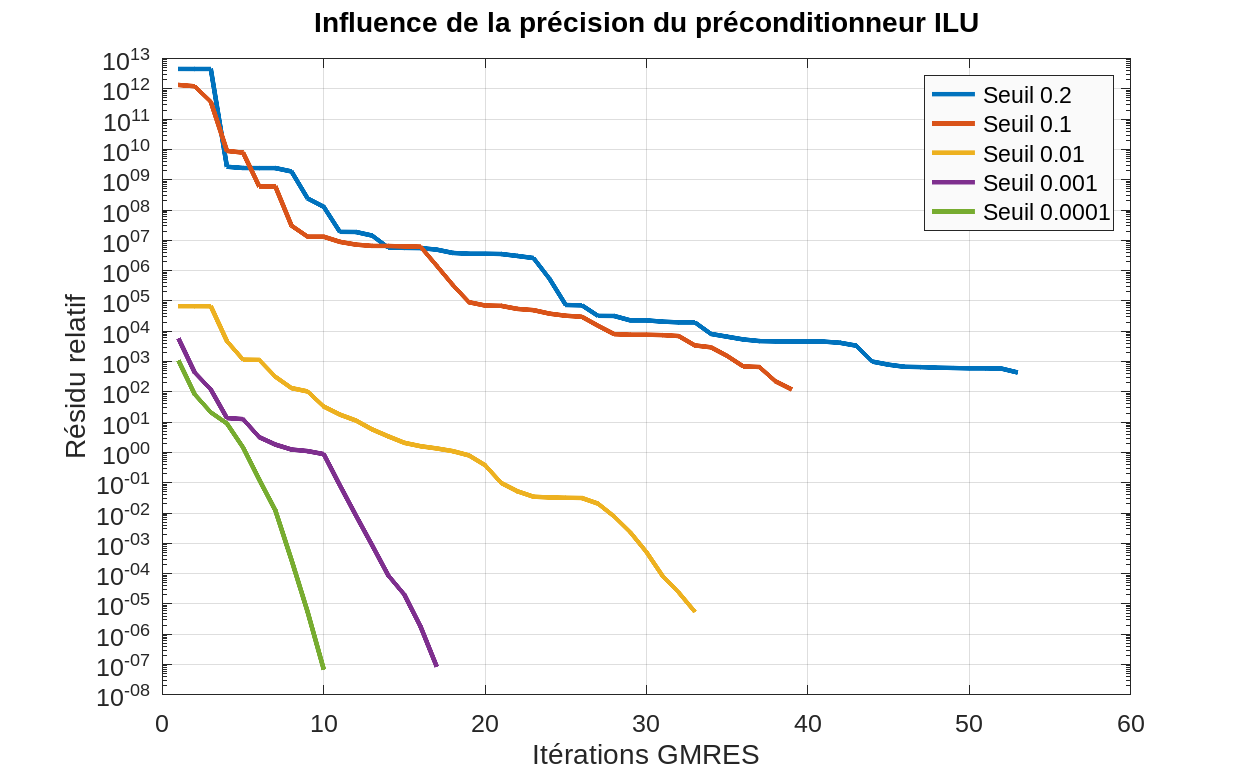
\includegraphics[width=\textwidth]{figures_rapport/Convergence_Pr_liminaire_ILU.png}
        \end{column}
    \end{columns}
\end{frame}

% 6. Phase 1 : Le Compromis Itérations-Remplissage et Dichotomie
\begin{frame}{Phase 1 : Compromis Itérations / Fill-in et Optimisation}
    \begin{columns}
        \begin{column}{0.45\textwidth}
            \textbf{Le Dilemme Classique :}
            \begin{itemize}
                \item À $\varepsilon = 10^{-5}$ : fill-in géant ($\approx 26\times$ plus d'éléments que la matrice originale).
                \item À $\varepsilon = 10^{-2}$ : fill-in proche de $1.0$ mais convergence plus lente.
            \end{itemize}
            \vspace{0.2cm}
            \textbf{Optimisation dichotomique (Ternaire) :}
            \begin{itemize}
                \item Minimisation de $J(\varepsilon) = \text{Time}_{\text{factorisation}}(\varepsilon) + (\text{Fill-in} \times \text{Iter})$.
                \item Recherche en $O(\log(1/\text{tol}))$.
                \item Optimum localisé à $\varepsilon \approx 1.75 \times 10^{-2}$ (fill-in $= 0.90$).
            \end{itemize}
        \end{column}
        
        \begin{column}{0.55\textwidth}
            \centering
            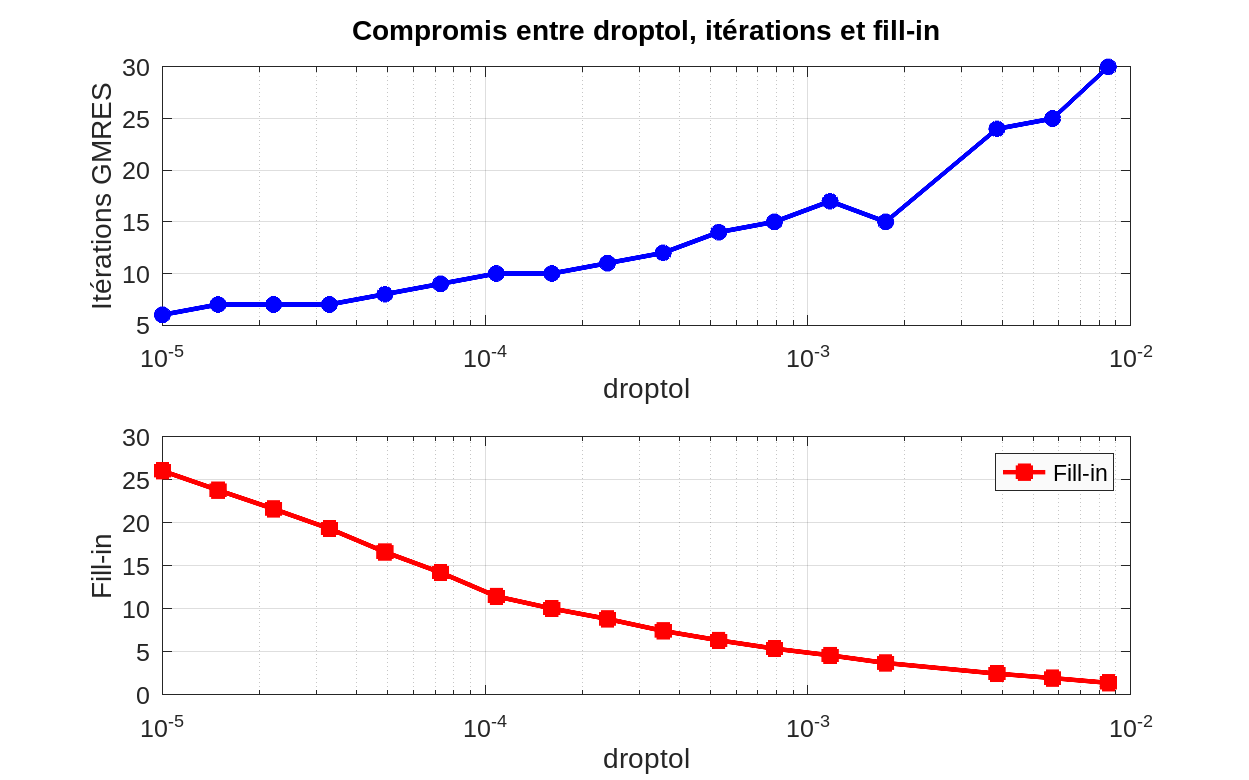
\includegraphics[width=0.95\textwidth]{figures_rapport/Compromis_It_rations_Fill_in.png}
        \end{column}
    \end{columns}
\end{frame}

% 7. Phase 1 : Limites de la Précision Basse Uniforme
\begin{frame}{Phase 1 : Instabilité d'une Précision Faible Uniforme}
    \begin{columns}
        \begin{column}{0.5\textwidth}
            \centering
            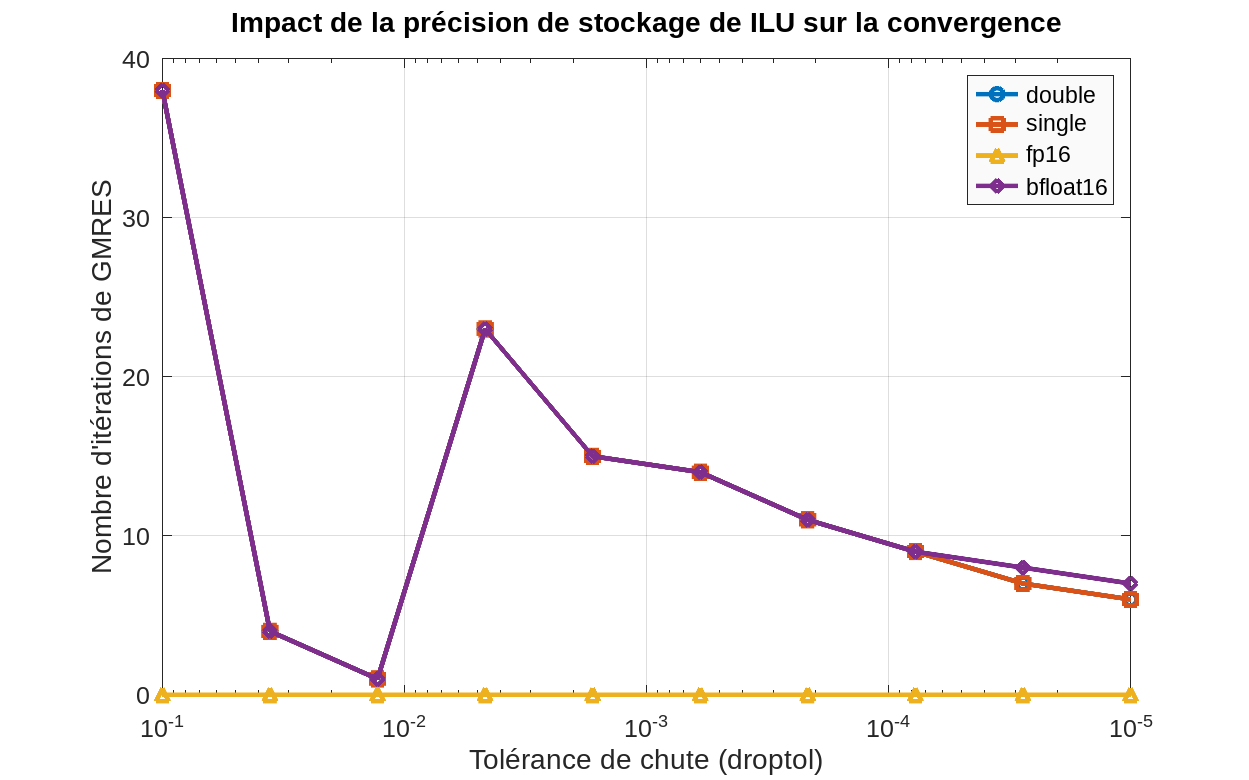
\includegraphics[width=\textwidth]{figures_rapport/It_rations_vs_Pr_cision_Simulation_.png}
            \begin{itemize}
                \item \textbf{FP16 Uniforme (ligne jaune à 0)} : Divergence complète sur toute la plage de tolérance stricte !
            \end{itemize}
        \end{column}
        
        \begin{column}{0.5\textwidth}
            \centering
            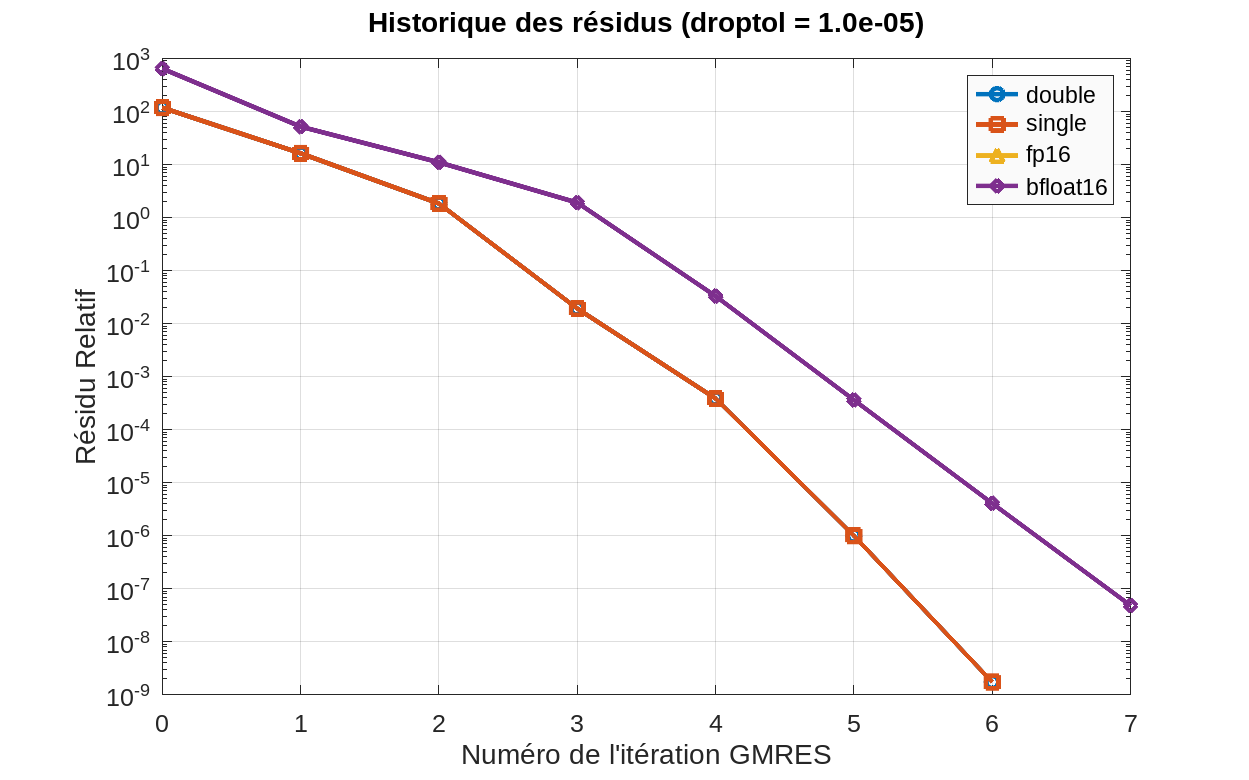
\includegraphics[width=\textwidth]{figures_rapport/Profil_de_Convergence_Simul_.png}
            \begin{itemize}
                \item \textbf{Historique à $\varepsilon = 10^{-5}$} : Le FP32 suit le FP64, mais le FP16 diverge instantanément (zéro point).
            \end{itemize}
        \end{column}
    \end{columns}
    \vspace{0.1cm}
    \centering \textit{Conclusion de la Phase 1 : Stocker tout en basse précision détruit le préconditionneur. Un choix sélectif et adaptatif est indispensable.}
\end{frame}

% 8. Phase 2 : Dérivation du Critère GEP Mixte
\begin{frame}{Phase 2 : Le Critère de Précision GEP Mixte}
    \begin{block}{Modèle d'Erreur d'Arrondi}
        Un élément conservé $x_{ij}$ stocké dans un format de précision $\mu_{ij}$ introduit une erreur locale $E_{ij}^{\text{round}} \le |x_{ij}|\,\mu_{ij}$.
    \end{block}
    
    Pour assurer que cette erreur ne dépasse pas le budget d'erreur déjà toléré par la colonne $j$ ($\varepsilon \|A_{\cdot,j}\|_2$), on déduit la contrainte suivante :
    
    \begin{columns}
        \begin{column}{0.5\textwidth}
            \begin{block}{Pour $U$ ($i \le j$) : Entrées Directes}
                $$|E_{ij}^{\text{round}}| \le |u_{ij}| \mu_{ij} \le \varepsilon \|A_{\cdot,j}\|_2$$
                $$\implies \mu_{ij} \le \frac{\varepsilon \|A_{\cdot,j}\|_2}{|u_{ij}|}$$
            \end{block}
        \end{column}
        
        \begin{column}{0.5\textwidth}
            \begin{block}{Pour $L$ ($i > j$) : Multiplicateurs amplifiés par le pivot}
                $$|E_{ij}^{\text{round}}| \le |l_{ij} u_{jj}| \mu_{ij} \le \varepsilon \|A_{\cdot,j}\|_2$$
                $$\implies \mu_{ij} \le \frac{\varepsilon \|A_{\cdot,j}\|_2}{|l_{ij} u_{jj}|}$$
            \end{block}
        \end{column}
    \end{columns}
    \vspace{0.3cm}
    \centering
    \textbf{Propriété clé :} Si l'élément est grand ou si le pivot $u_{jj}$ est grand $\implies$ $\mu_{ij}$ doit être très petit (FP64 requis). Si l'élément est proche du seuil $\implies$ $\mu_{ij}$ grand (FP16 autorisé).
\end{frame}

% 9. Algorithme GEP Mixte \& Complexité
\begin{frame}{Algorithme GEP Mixte et Complexité}
    \begin{columns}
        \begin{column}{0.6\textwidth}
            \textbf{L'Algorithme :}
            \begin{enumerate}
                \item Durant l'élimination de Gauss, pour chaque coefficient calculé au-dessus du seuil $\varepsilon\|A_{\cdot,j}\|_2$, on calcule sa cible $\tau_{ij}$.
                \item On lui attribue le format matériel le plus économique vérifiant $\mu_{ij} \le \tau_{ij}$ :
                $$\text{Cible } \tau_{ij} \ge u_{16} \implies \textbf{FP16 (Half)}$$
                $$u_{16} > \tau_{ij} \ge u_{24} \implies \textbf{FP24}$$
                $$u_{24} > \tau_{ij} \ge u_{32} \implies \textbf{FP32}$$
                $$u_{32} > \tau_{ij} \ge u_{48} \implies \textbf{FP48}$$
                $$u_{48} > \tau_{ij} \implies \textbf{FP64 (Double)}$$
            \end{enumerate}
        \end{column}
        
        \begin{column}{0.4\textwidth}
            \begin{block}{Complexité arithmétique additionnelle}
                \begin{itemize}
                    \item \textbf{Normes des colonnes} : Calculées 1 fois au départ $\implies 2\,\text{nnz}(A)$ ops.
                    \item \textbf{Évaluation par élément} : 
                    \begin{itemize}
                        \item Pour $U$ : 1 division.
                        \item Pour $L$ : 1 multiplication + 1 division.
                    \end{itemize}
                    \item \textbf{Coût global} : $O(\text{nnz}(L) + \text{nnz}(U))$, soit seulement 1 à 2 flops supplémentaires par élément stocké.
                    \item \textbf{Totalement négligeable} devant le coût $O(n^3)$ de la factorisation ou de GMRES !
                \end{itemize}
            \end{block}
        \end{column}
    \end{columns}
\end{frame}

% 10. GEP Mixte : Robustesse et Préservation de la Sparsité
\begin{frame}{Résultats : Robustesse spectrale et Remplissage}
    \begin{columns}
        \begin{column}{0.45\textwidth}
            \textbf{Observations :}
            \begin{itemize}
                \item \textbf{Gauche (Itérations)} : GEP Mixte (courbe bleue) se superpose parfaitement aux itérations du FP64 de référence. Il n'y a \textbf{aucune perte de convergence}, contrairement au FP16 uniforme qui diverge.
                \item \textbf{Droite (Fill-in)} : Le facteur de remplissage est rigoureusement identique. La sélection du format intervient après le dropping arithmétique, préservant le profil de creux de la matrice.
            \end{itemize}
        \end{column}
        
        \begin{column}{0.55\textwidth}
            \centering
            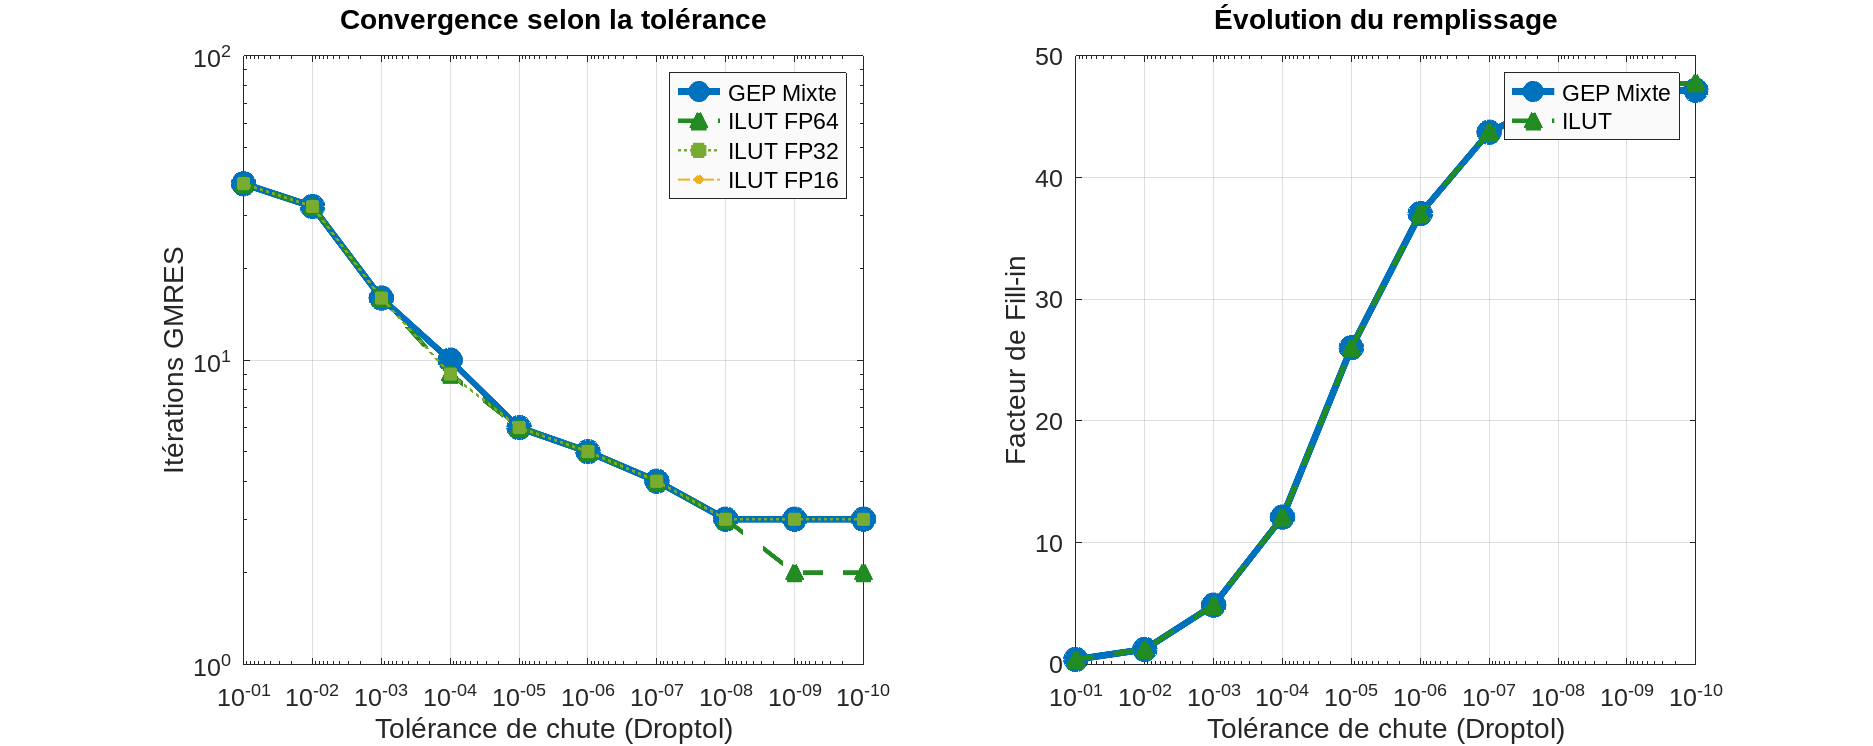
\includegraphics[width=\textwidth]{figures_rapport/Convergence_et_Fill_in.png}
        \end{column}
    \end{columns}
\end{frame}

% 11. Distribution des Formats de Précision dans GEP Mixte
\begin{frame}{Résultats : Allocation Dynamique des Formats}
    \begin{columns}
        \begin{column}{0.45\textwidth}
            \textbf{Analyse physique de l'allocation :}
            \begin{itemize}
                \item \textbf{Aux tolérances strictes ($\le 10^{-4}$)} : Plus de \textbf{90\% des éléments} sont alloués en \textbf{FP16} ! Seuls les pivots et quelques éléments critiques sont en \textbf{FP24}.
                \item \textbf{Aux tolérances lâches ($\ge 10^{-1}$)} : Le FP16 chute à 19\% et le \textbf{FP24 domine à 81\%}. 
                \item \textbf{Pourquoi ?} À $10^{-1}$, seuls les pivots géants sont conservés. Étant très grands, ils demandent une précision stricte ($\mu_{ij}$ petit), forçant le passage en FP24 pour éviter des erreurs catastrophiques sur les pivots.
            \end{itemize}
        \end{column}
        
        \begin{column}{0.55\textwidth}
            \centering
            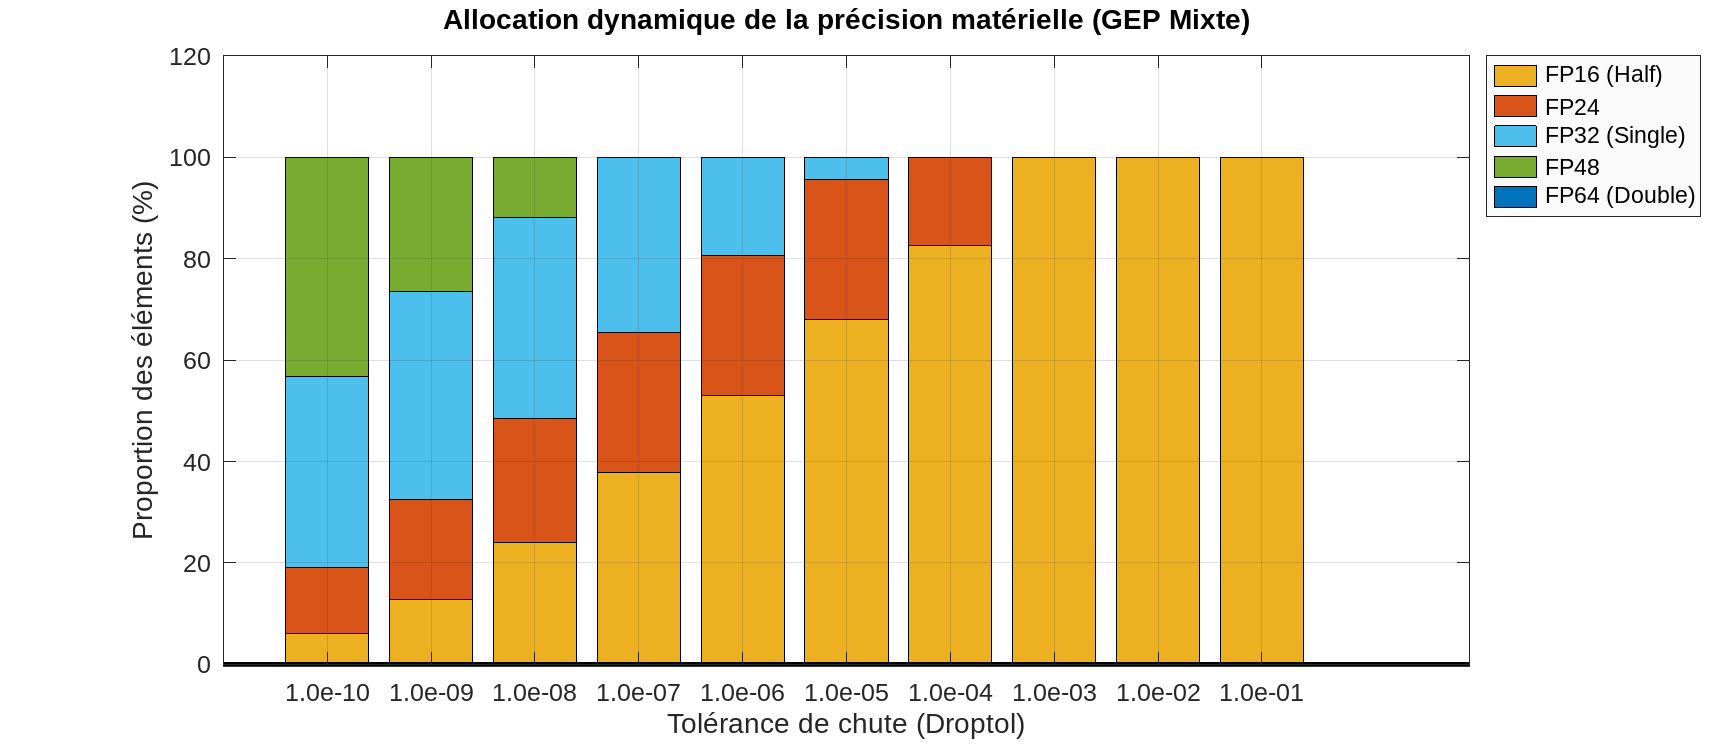
\includegraphics[width=0.95\textwidth]{figures_rapport/Distribution_des_formats_de_pr_cision.png}
        \end{column}
    \end{columns}
\end{frame}

% 12. Gain en Empreinte Mémoire
\begin{frame}{Résultats : Compression de l'Empreinte Mémoire}
    \begin{columns}
        \begin{column}{0.45\textwidth}
            \textbf{Analyse de la taille mémoire (KB) :}
            \begin{itemize}
                \item \textbf{Régime optimal ($\varepsilon = 10^{-5}$)} :
                \begin{itemize}
                    \item Stockage Standard FP64 : \textbf{2640 KB}.
                    \item Stockage GEP Mixte : \textbf{700 KB}.
                    \item \textbf{Facteur de compression : 3.8$\times$ !}
                \end{itemize}
                \item GEP Mixte colle à l'encombrement du FP16 pur pour les tolérances courantes, tout en évitant sa divergence.
                \item Permet de charger des préconditionneurs de très grande taille en mémoire vive limitée.
            \end{itemize}
        \end{column}
        
        \begin{column}{0.55\textwidth}
            \centering
            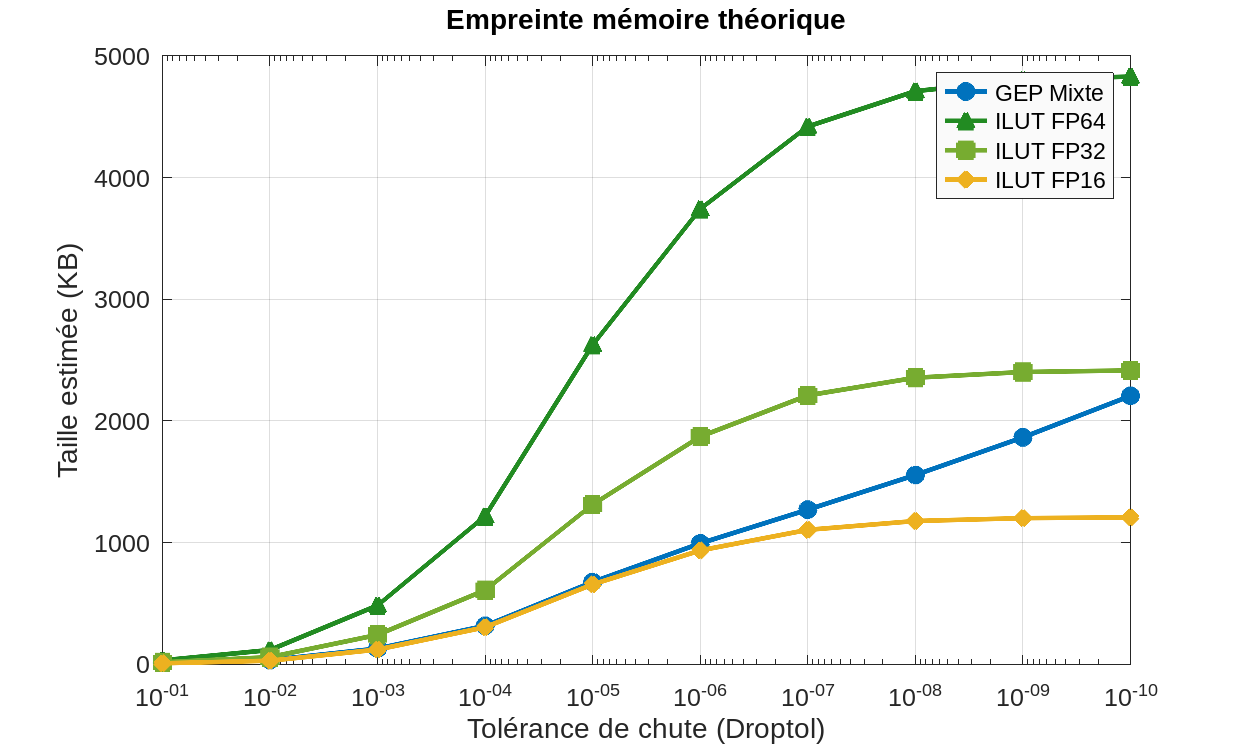
\includegraphics[width=0.95\textwidth]{figures_rapport/Empreinte_M_moire.png}
        \end{column}
    \end{columns}
\end{frame}

% 13. Profils de Performance Dolan-Moré : Efficacité Mémoire
\begin{frame}{Résultats : Profil de Performance Dolan-Moré -- Mémoire}
    \begin{columns}
        \begin{column}{0.5\textwidth}
            \centering
            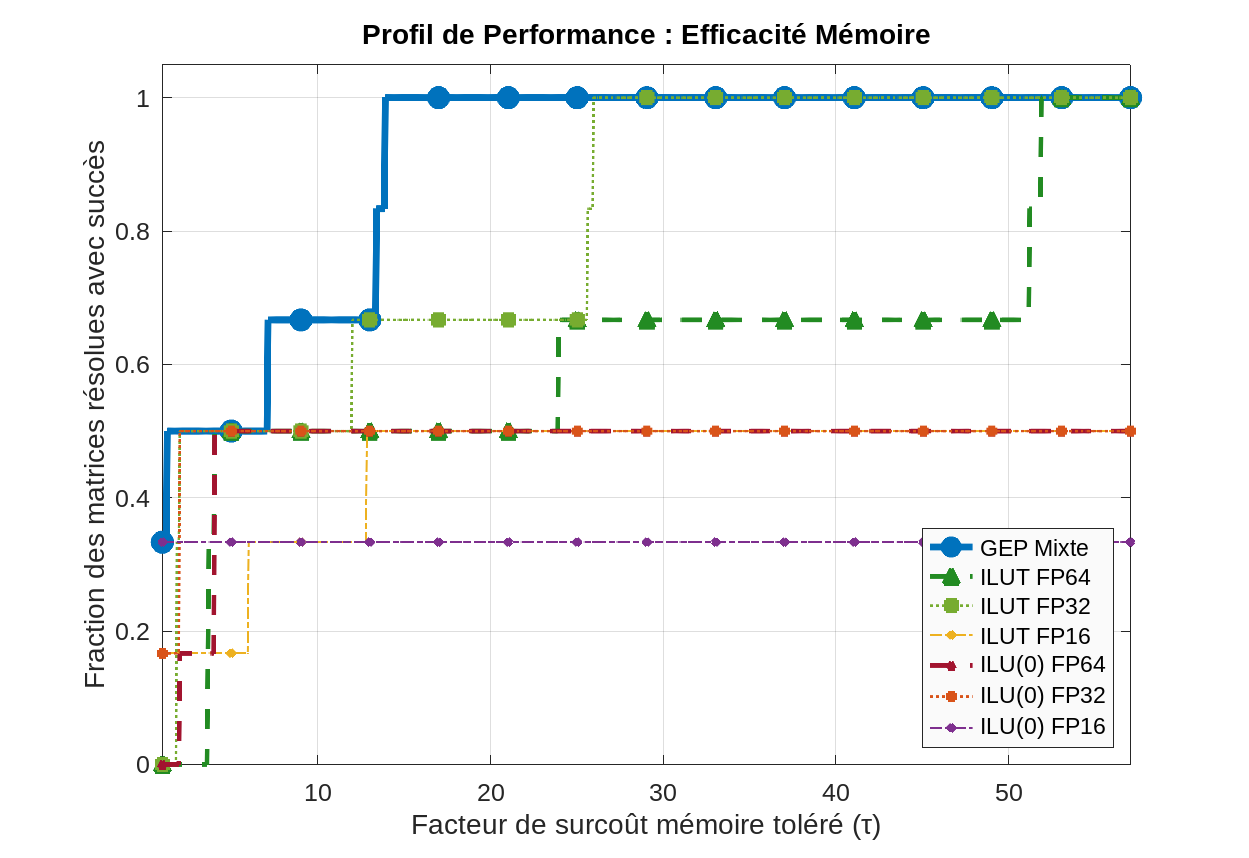
\includegraphics[width=0.85\textwidth]{figures_rapport/Profil_de_Performance_M_moire.png}
            \begin{itemize}
                \item \textbf{Profil Global (avec ILU(0))} : GEP Mixte (bleu) domine largement tous les solvers robustes en efficacité mémoire.
            \end{itemize}
        \end{column}
        
        \begin{column}{0.5\textwidth}
            \centering
            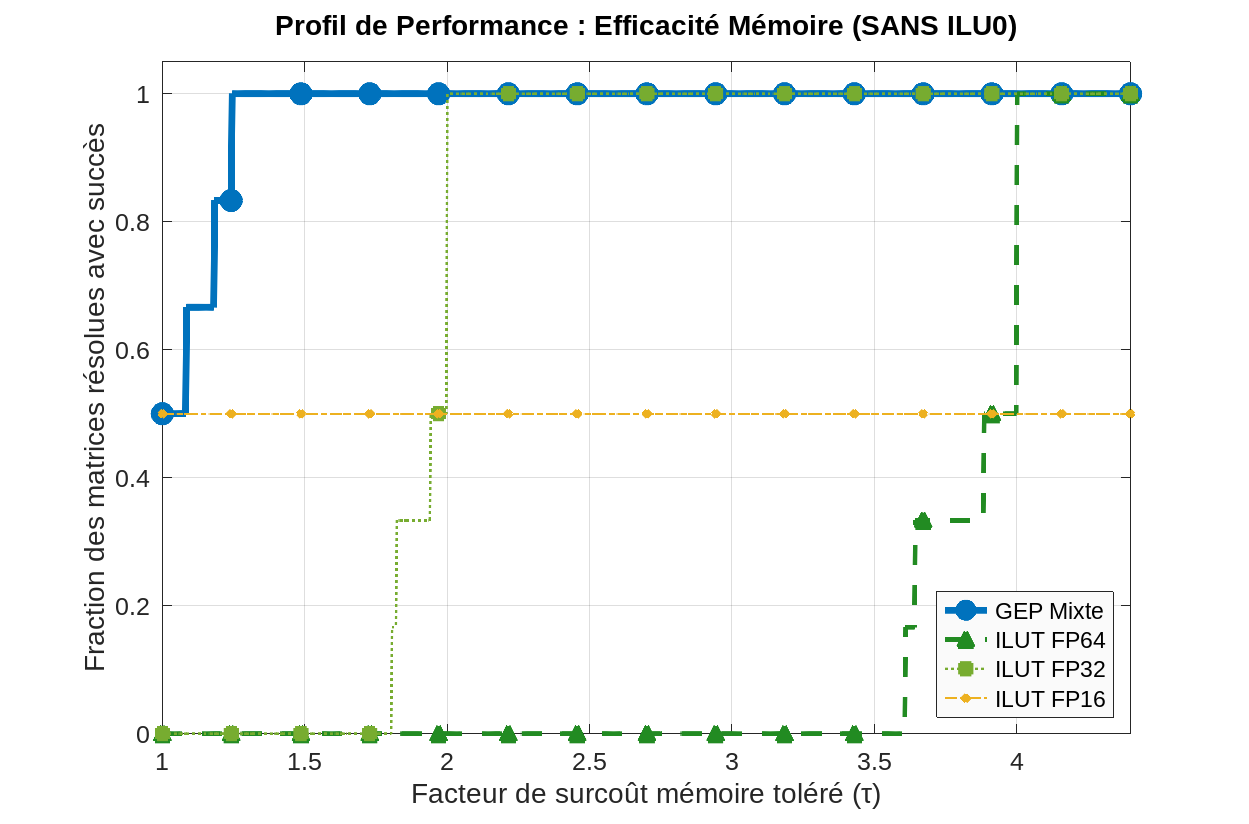
\includegraphics[width=0.85\textwidth]{figures_rapport/Profil_de_Performance_M_moire_SANS_ILU0_.png}
            \begin{itemize}
                \item \textbf{Profil sans ILU(0)} : À $\tau=1$, GEP Mixte partage la tête avec FP16. Mais FP16 stagne à 0.50 (divergence sur 3/6 matrices), tandis que GEP Mixte résout \textbf{100\% des cas}.
            \end{itemize}
        \end{column}
    \end{columns}
    \vspace{0.1cm}
    \centering \textit{GEP Mixte atteint $\rho = 1.0$ à $\tau \approx 1.3$ (à peine 30\% plus lourd que le FP16 brut), garantissant robustesse et compacité.}
\end{frame}

% 14. Profils de Performance Dolan-Moré : Robustesse Itérations
\begin{frame}{Résultats : Profil de Performance Dolan-Moré -- Itérations}
    \begin{columns}
        \begin{column}{0.5\textwidth}
            \centering
            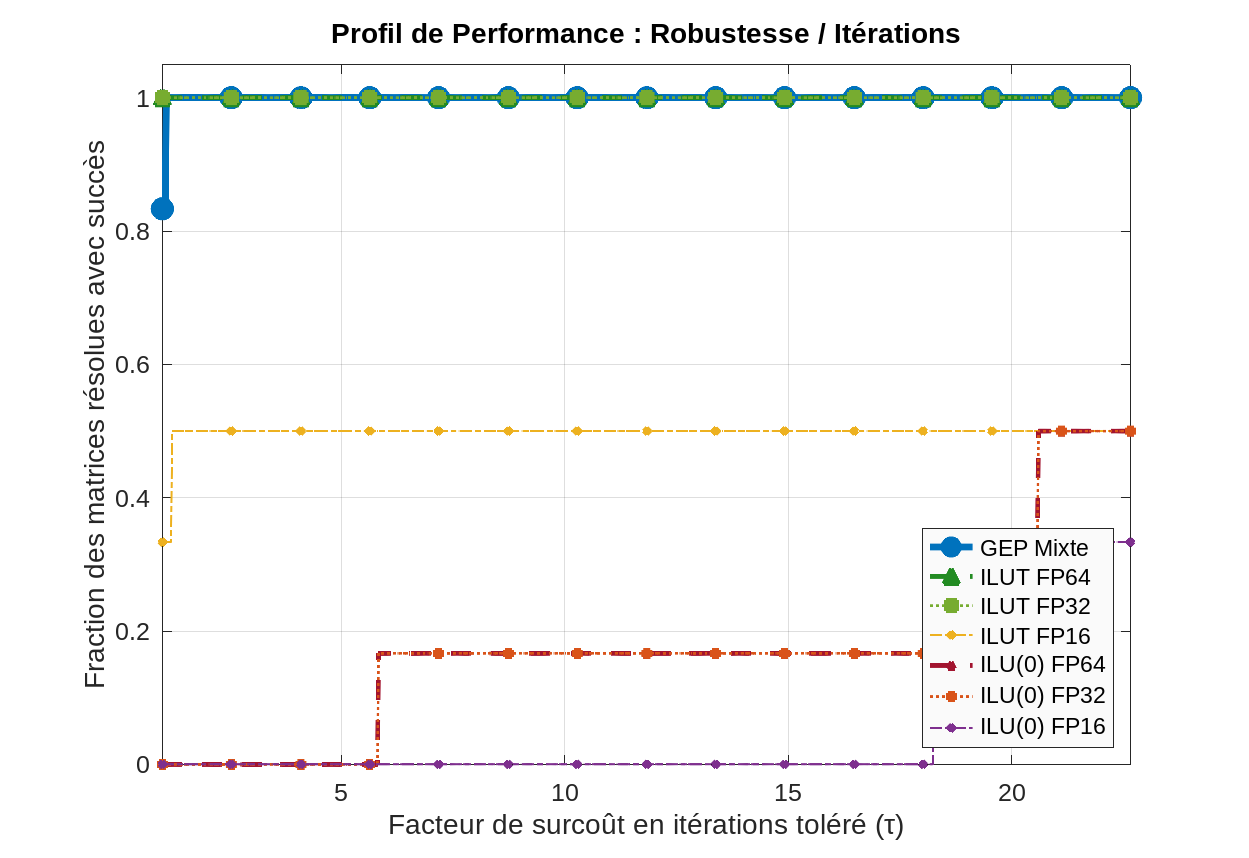
\includegraphics[width=0.85\textwidth]{figures_rapport/Profil_de_Performance_It_rations.png}
            \begin{itemize}
                \item GEP Mixte (bleu) offre exactement la même robustesse face aux itérations que les solvers double précision (FP64).
            \end{itemize}
        \end{column}
        
        \begin{column}{0.5\textwidth}
            \centering
            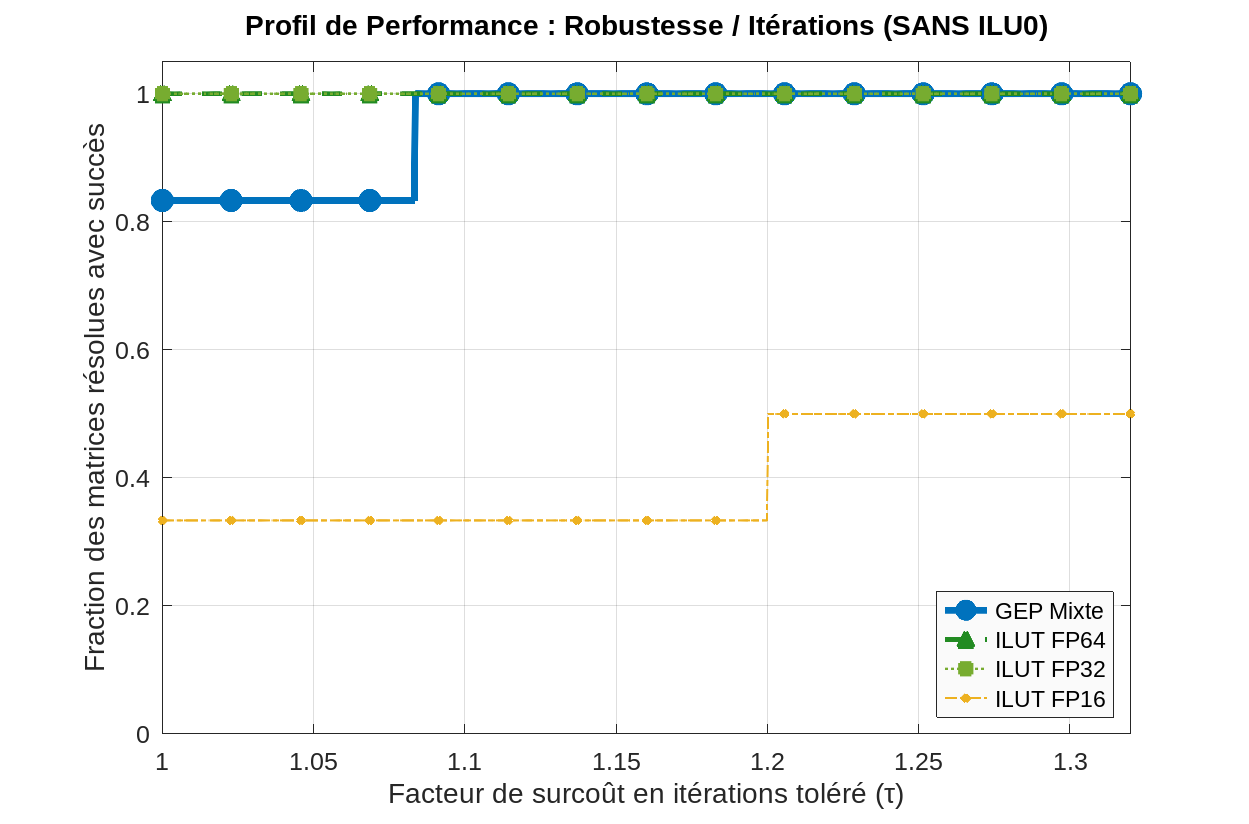
\includegraphics[width=0.85\textwidth]{figures_rapport/Profil_de_Performance_It_rations_SANS_ILU0_.png}
            \begin{itemize}
                \item GEP Mixte atteint $\rho = 1.0$ à $\tau \approx 1.09$. Soit au pire un surcoût d'itérations de seulement \textbf{9\%} sur une seule matrice, et \textbf{0\% d'écart sur les 5 autres}.
            \end{itemize}
        \end{column}
    \end{columns}
    \vspace{0.1cm}
    \centering \textit{La perte d'information liée à la compression est numériquement indétectable par le solveur GMRES.}
\end{frame}

% 15. Conclusion \& Perspectives
\begin{frame}{Conclusion \& Travaux Futurs}
    \begin{block}{Principaux acquis de l'étude}
        \begin{enumerate}
            \item \textbf{Critère de précision constructif} reliant rigoureusement l'erreur d'arrondi locale au budget de dropping de la colonne, avec gestion de l'amplification par les pivots.
            \item \textbf{Forte compression mémoire de 3.8$\times$} par rapport au FP64 uniforme.
            \item \textbf{Robustesse mathématique absolue (100\% de convergence)} préservée sur des cas d'ingénierie difficiles (SuiteSparse), là où la précision basse uniforme échoue.
            \item \textbf{Zéro surcoût arithmétique réel} lors de la factorisation ($O(\text{nnz})$ additionnel).
        \end{enumerate}
    \end{block}
    
    \vspace{0.3cm}
    \begin{columns}
        \begin{column}{0.5\textwidth}
            \textbf{Limitations actuelles :}
            \begin{itemize}
                \item Utilisation de structures denses pour la factorisation active.
                \item Les formats personnalisés (FP24, FP48) sont simulés de manière logicielle.
            \end{itemize}
        \end{column}
        
        \begin{column}{0.5\textwidth}
            \textbf{Travaux futurs :}
            \begin{itemize}
                \item Co-design matériel : Implémenter GEP Mixte sur puces dédiées (FPGA/ASIC custom bit-width).
                \item Intégration en structures creuses compressées natives.
            \end{itemize}
        \end{column}
    \end{columns}
\end{frame}

\end{document}
